\documentclass[a4j,10.5pt]{jreport}
\usepackage[dvipdfmx]{graphicx}
\usepackage{amssymb}
\usepackage{amsmath}
\usepackage{float}
\usepackage{here}


% \usepackage{tabularx}
% \usepackage{multirow}
% \usepackage{slashbox} default commented out
\usepackage{cite}
% \usepackage{supertabular}
% \usepackage{jtygm} default commented out

\makeatletter %% プリアンブルで定義する場合は必須

% \setcounter{secnumdepth}{5}

%\newcommand{\figcaption}[1]{\def\@captype{figure}\caption{#1}}
%\newcommand{\tblcaption}[1]{\def\@captype{table}\caption{#1}}



%---------------------------------------------------------------------
%\setcounter{topnumber}{5}%    ページ上部の図表は 5 個まで
%\def\topfraction{1.00}%       ページの上 1.00 まで図表で占めて可
%\setcounter{bottomnumber}{5}% ページ下部の図表は 5 個まで
%\def\bottomfraction{1.00}%    ページの下 1.00 まで図表で占めて可
%\setcounter{totalnumber}{10}% ページあたりの図表は 10 個まで
\def\textfraction{0.2}%        ページのうち本文が占める割合の下限
%        これを 0 にすると本文が 1 行だけのページが出来る
%        0.04 くらいにするとS 1 行だけのページは防げる
%        0.1 くらいが良いかも知れない
\def\floatpagefraction{0.8}%   図表だけのページは少ないかも
                           %   これだけを図表が占める
%---------------------------------------------------------------------

\renewcommand{\bibname}{参考文献}


\makeatother %% プリアンブルで定義する場合は必須

\begin{document}

\begin{titlepage}

\vspace{40mm}
\begin{center}
{\Large 平成31年度\\卒業論文}\\[80mm]
\end{center}

\begin{center}
{\huge 歩行時における足の接地推定}\\[80mm]
\end{center}

\begin{flushright}
{\large s163043 鈴木健太}\\[1mm]
{\large 平成28年度入学}\\[1mm]
{\large 島根大学 総合理工学部 数理・情報システム学科}\\[1mm]
{\large 情報システムコース}\\[8mm]
{\large 主指導教員: 平川 正人 教授}\\[3mm]
{\large 提出日:令和2年1月24日}\\%
\end{flushright}
\end{titlepage}

\newpage
% \pagenumbering{roman}

\chapter*{概要}
人の動作の計測や解析は運動学やヒューマンコンピュータインタラクションなどの様々な分野に応用されている.特に,人の動作の中でも歩容解析は最も注目されている研究テーマの一つである.体組成の推定\cite{cite1},個人識別,トレーニングやリハビリテーション,転倒予防などへの応用が図られている.歩容解析にあたって用いられるパラメータには大きく分けて次の2つがある.ひとつは空間的パラメータであり,ステップ長やスライド長などが含まれる.もうひとつは時間的パラメータである.これは遊脚期や両脚支持期\cite{cite2}など,足の位置に着目し歩行周期を分類したパラメータである.

本研究では,姿勢推定ライブラリの1つであるPoseNetを用いて,
歩行時における各特徴点の値を解析して両脚支持相を抽出することを目指す.
\addcontentsline{toc}{chapter}{概要}

\section*{Abstract}
Measurement and analysis of human movements have been applied to various fields such as kinematics and human-computer interaction. In the field of human motion analysis, gait analysis is one of the most attractive research topics and can be used for estimation of, for example, human body composition, personal identification, training and rehabilitation, and fall prevention. When performing gait analysis, certain parameters related to body parts are observed. These parameters are divided into the following two: One is spatial parameters which include step length, slide length, etc. The other is temporal parameters that classify each stage by focusing on the position of the foot in one cycle of walking, such as a swing phase and a double supporting phase.

In this study, we use PoseNet, one of the pose estimation libraries, to analyze the value of each keypoints during walking and extract the double legs supporting phase in a non-invasive manner. In experiments, it was shown that Fourier analysis could be used to extract the double legs supporting phase from information obtained from posture estimation.
\pagenumbering{roman}

\tableofcontents

\listoftables %表目次

\listoffigures %図目次

\baselineskip = 8mm

\clearpage

\pagenumbering{arabic}


% 必要に応じてchapter,sectionを追加・変更する.

\chapter{はじめに}
\section{研究背景}
人の動作の計測,解析は運動力学やヒューマンコンピュータインターフェースなど様々な分野に応用が期待されている.特に,人の動作の中でも歩容解析は,最も注目されている研究テーマの一つである.また,歩容解析に関わる研究の多くはセンサ情報や複数台のカメラからの情報を利用している.しかし,この方法では複数人を対象とした解析を同時に行うことが難しく,さらに利用コストも上昇しやすいという問題点がある.この問題を解決すべく,Webブラウザ上で動作し同時に複数人の姿勢推定が可能なPoseNetを用いて歩容解析を行う.
\section{研究目的}
本研究では,姿勢推定ライブラリの1つであるPoseNetを用いて,
歩行時における各特徴点の値を解析し,歩行パラメータの内の時間的パラメータである両脚支持相を抽出することを目指す.

\section{本論文の構成}
本論文の構成は以下の通りである.第2章では関連研究について紹介し,第3章は本研究の手法について述べる.次に,第4章では本手法の評価をする.最後に第5章では今後の展開について記述する.

\chapter{関連研究}
\section{歩行位相分割に関する研究}
安川らの研究\cite{yasukawa}によると,左右足の状態について相互制約を持った歩行位相分割アルゴリズムを,位相分割手法のひとつである動的計画法を用いた区分線形近似手法の改良を行うことで開発した.この歩行位相分割アルゴリズムは,片麻痺のように非対称な歩容に対しても精度を保ち,4相に歩行周期を分割している.
\section{歩容解析の応用に関する研究}
歩容解析の応用は,歩行動作が身体動作の中でも重要な位置を占めていることから盛んに研究されている.廖ら\cite{cite1}の研究では,体組成に強く関わる運動機能の評価に歩行動作が用いられることを利用し,歩行映像の解析を行うことによって体組成を推定する手法を提案している.堀ら\cite{hori}の研究では,歩行認識に関するこれまでの研究が視覚情報やセンサ情報を用いており,プライバシーの問題やシステムの複雑さを指摘し,音響情報のみを用いた個人識別システムの提案を行っている.Funkら\cite{funk}の研究のようにセンサデータを教師データとした機械学習ベースの歩容解析も広く研究されている.


\chapter{提案手法}
\section{データ収集}
入力映像としては歩行者が単独で,自然な歩行を足全体が写るように横方向から撮影したものを用いた.今回の研究では,歩行時に大きく位置が変動する膝,足首,手首を特徴点として選び,PoseNetを用い姿勢推定を行い,手首,膝,足首の左右計6箇所の特徴点からデータを収集した.サンプリングレートは$28\,\mathrm{Hz}$である.PoseNetは機械学習用ライブラリのtensorflow.jsの一部なのでjavascript上で動作する.よって今回の研究では,図\ref{fig:datecollect}のようにlocal環境でjavascriptプログラムを実行し,歩行時の映像から特徴点の座標を推定し,csv形式で保存した.収集されたデータはそれぞれパラメータとして時間,x座標,y座標の3つを持つ.
\begin{figure}[H]
  \centering
  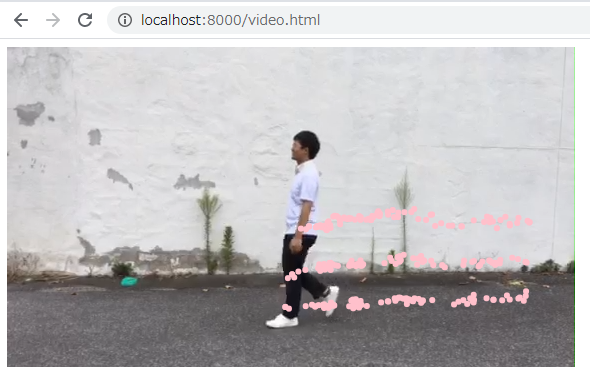
\includegraphics[width=10cm]{figs/datacollect1.png}
  \caption{歩行映像からの歩行特徴データの取得}\label{fig:datecollect}
\end{figure}

\newpage
\section{データ分析}
データ分析に先立ち,撮影した歩行を1フレームレートごとに停止し確認したところ,周波数$1.47\,\mathrm{Hz}$,周期$0.68\,\mathrm{秒}$であった.これを考慮し分析を行う.
左右それぞれの手首,膝,足首の位置データを時系列でグラフ化したものが図\ref{fig:originaldata}である.この状態から直接は周期性が見出せないので,歩行動作の特徴からデータ処理を行う.\cite{gait_analyse}によると,歩行周期において立脚期の初期状態イニシャルコンタクト(床への足接地の瞬間)と遊脚期の最後であるターミナルスタンス(床に足が着く直前)の2つの相では足関節はニュートラル・ゼロ・ポジションである.ニュートラル・ゼロ・ポジションとは,足がまっすぐに伸び,左右の膝の間の距離が最大になる状態を指している.このことを踏まえ,収集した特徴点に対し,手首,膝,足首のそれぞれについて左右部位間のユークリッド距離$L$を以下の式で求めた.処理結果を図\ref{fig:lengthdata}に示す.

\begin{equation}
  L = \{(x_{left} - x_{right})^2 + (y_{left} - y_{right})^2\}
\end{equation}

図\ref{fig:lengthdata}より,一定の間隔で頂点が見られることから周期性があると推測される.ここで,周期性を確かめるべく左右部位間の距離の自己相関を調べる.用いる自己相関関数は以下の式(\ref{equ:acf})の通りである.ここでは相関係数を$\rho$,ある時間$t_i$における左右部位間の距離を$L_{t_i}(i\in \mathbb{N})$,任意の正の整数を$\tau$,距離の平均を$\Bar{L}$とする.
\begin{equation}\label{equ:acf}
    \rho_\tau = \frac{\sum_{i=1}^{n}(L_{t_i}-\Bar{L})(L_{t_{i+\tau}}-\Bar{L})}
    {\sqrt{\sum_{i=1}^{n}(L_{t_{i}}-\Bar{L})^2(L_{t_{i+\tau}}-\Bar{L})^2}}
\end{equation}
$\tau$は元信号からのずれを表している.自己相関係数を$\tau$をもとに整理すると,図\ref{fig:acf}に示すようなコレログラムが得られる.図\ref{fig:acf}中の破線は$95\%$信頼区間を表している.よって膝間の距離において$\tau=19$で相関があることが示された.このため,PoseNetからのデータには周期があるといえる.更により細かく周期を求めるためフーリエ解析を行う.
\newpage
\section{フーリエ解析}
手首,膝,足首のそれぞれの取得データについてフーリエ変換を行い,歩行周期も考慮し周波数成分の分析を行った.フーリエ変換を用いることによって,歩行周期を周波数成分に分解でき,元のデータでは判別がしづらい特徴を分析可能である.フーリエ変換には高速フーリエ変換(FFT)と呼ばれるものを用いた.これはデータ数を$2^n$個に制限することで高速に処理できるアルゴリズムである.高速フーリエ変換の式を以下に示す.
\begin{equation}
    F(t)=\sum_{x=0}^{N-1}f(x)e^{-i\frac{2\pi tx}{N}}
\end{equation}
ここで,$f(x)$と$F(x)$は複素関数である.収集されたデータから$2^n$の範囲で高速フーリエ変換を行う際に,データの両端を滑らかにするための窓関数にハミング窓を利用する.
フーリエ変換の結果を図\ref{fig:frequency}に示す.膝については$1.30\,\mathrm{Hz} $,言い換えると$0.77\,\mathrm{秒}$の周期特徴,足首については$1.52\,\mathrm{Hz}$($0.66\,\mathrm{秒}$周期)という結果が得られた.

\begin{figure}
    \centering
    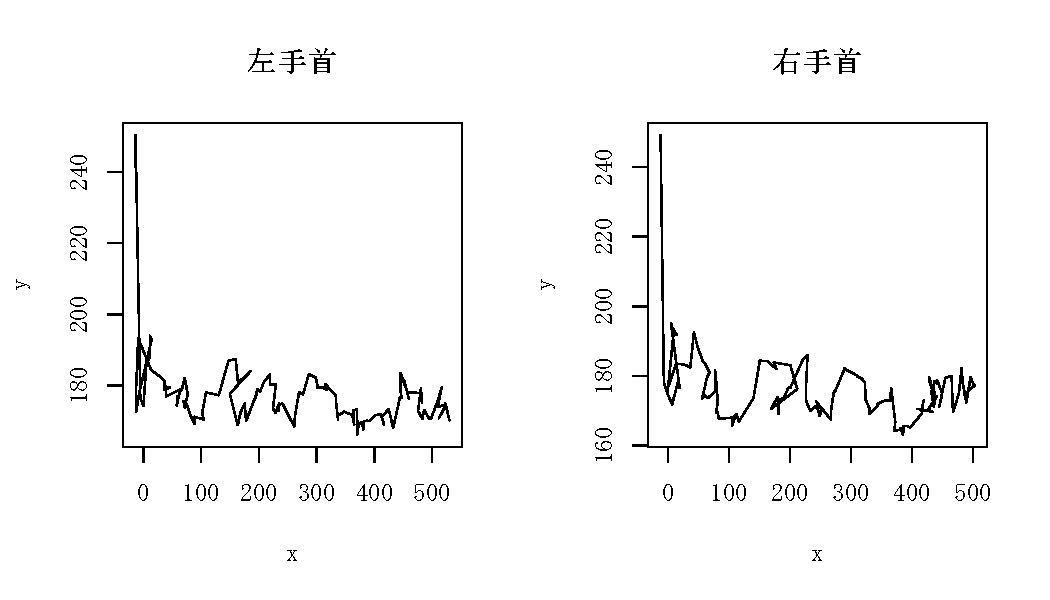
\includegraphics[width=0.88\linewidth]{figs/original_wrist.pdf}
    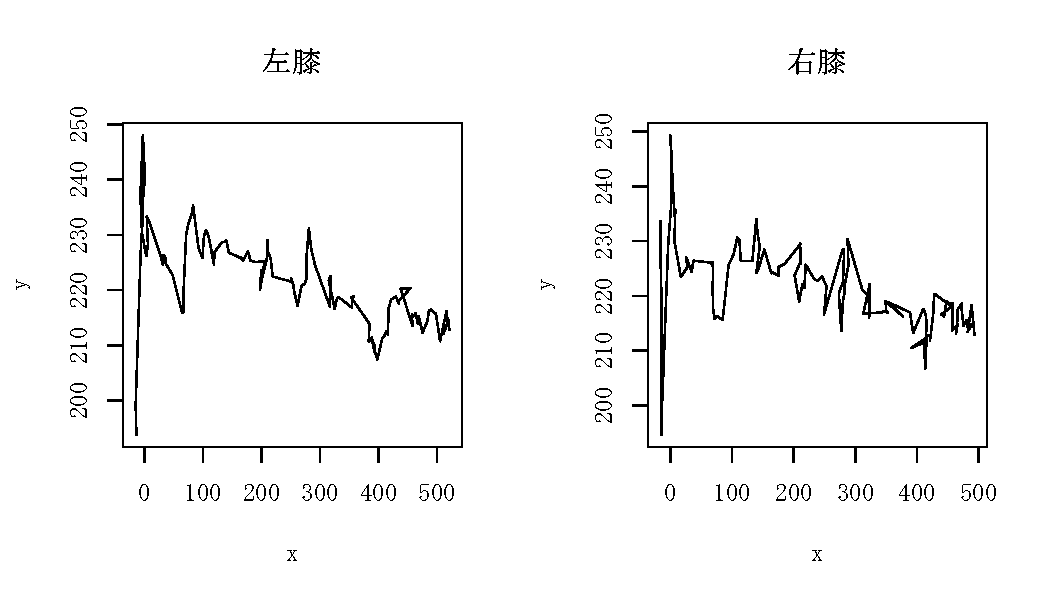
\includegraphics[width=0.88\linewidth]{figs/original_knee.pdf}
    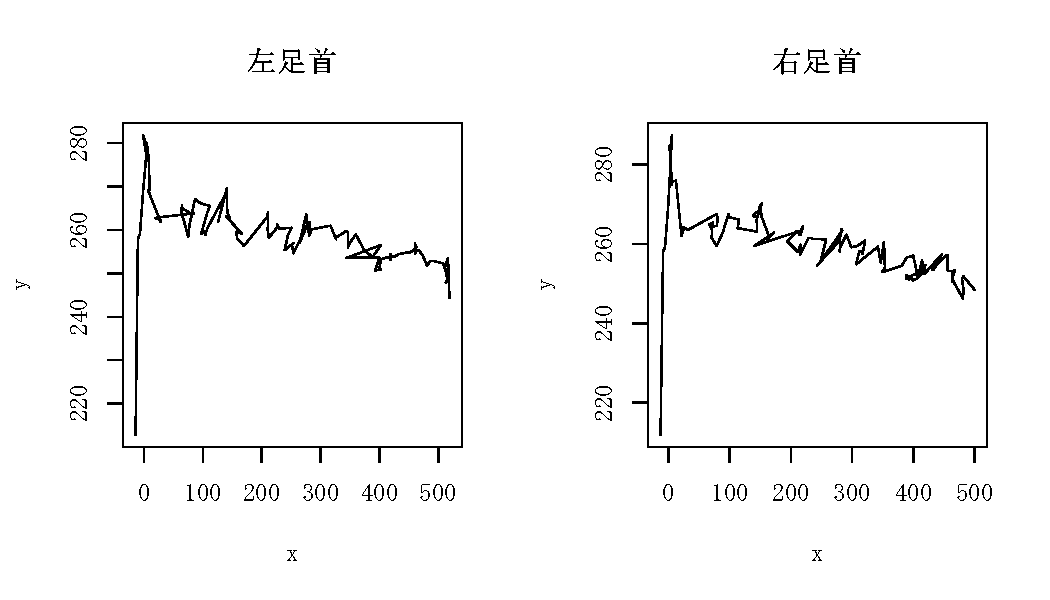
\includegraphics[width=0.88\linewidth]{figs/original_ankle.pdf}
    \caption{元データ}
    \label{fig:originaldata}
\end{figure}
\begin{figure}
    \centering
    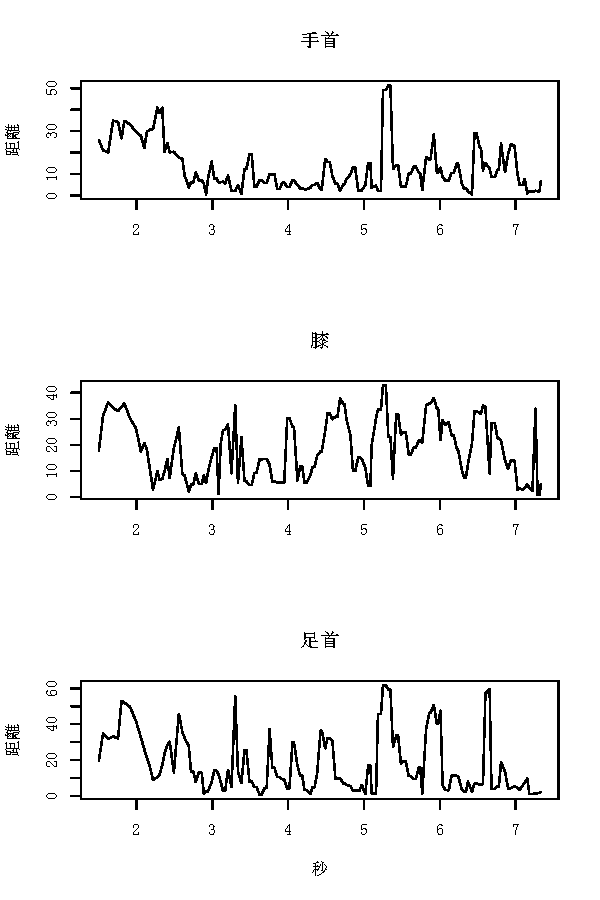
\includegraphics[width=\linewidth]{figs/distance.pdf}
    \caption{左右関節間距離}
    \label{fig:lengthdata}
\end{figure}
\begin{figure}
    \centering
    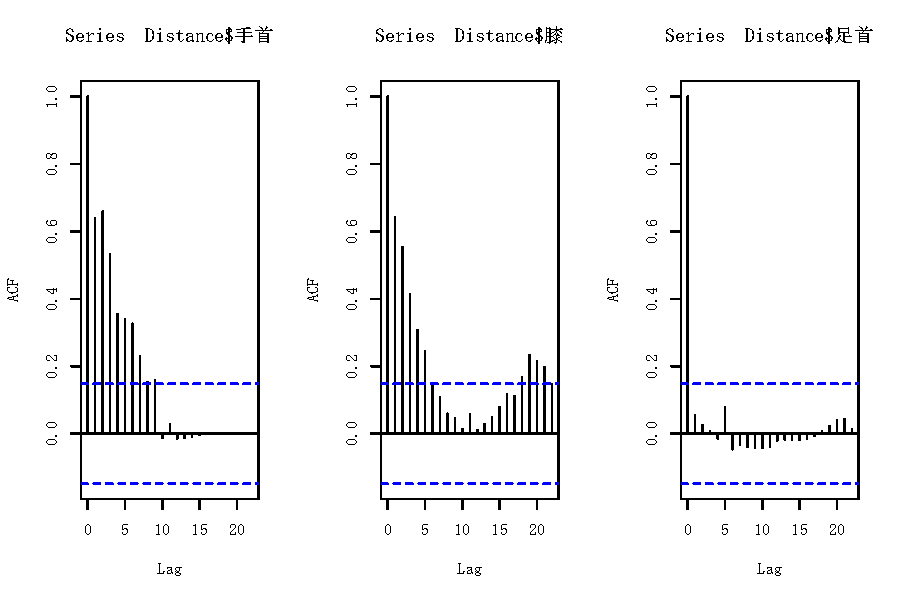
\includegraphics{figs/acf.pdf}
    \caption{コレログラム}
    \label{fig:acf}
\end{figure}
\begin{figure}
    \centering
    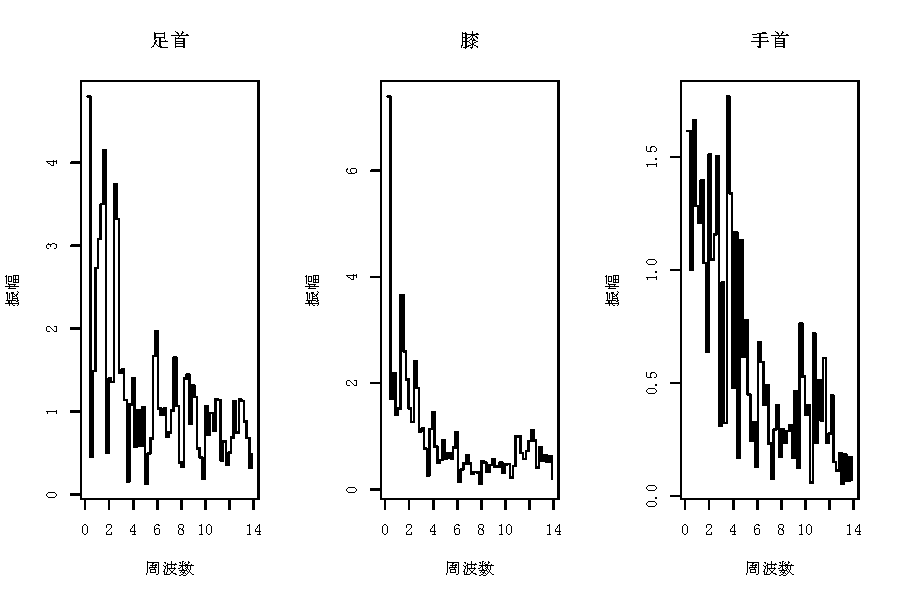
\includegraphics{figs/frequency.pdf}
    \caption{フーリエ変換結果}
    \label{fig:frequency}
\end{figure}

\chapter{評価}

\section{フーリエ解析}
4つの歩行映像に対して3章で説明した手法を用いて解析を行った.解析結果の歩行周期$\nu_i$と目視で確認した周期$\nu_t$との誤差率$\delta_i =|(\nu_i-\nu_t)/\nu_t|\times100\%$を表\ref{tab:結果}に整理する.data2については,外れ値が多く$\delta_2$は求められなかった.data2以外については,膝より足首の方が実際の歩行周期にあっていることがわかった.
\begin{table}[H]
\caption{解析結果} \label{tab:結果}
\vspace{5mm}
  \centering
  \begin{tabular}{c||ccc}
    \hline
            & 目視[秒] & 膝誤差率$\delta_1$[$\%$]& 足首誤差率$\delta_2$[$\%$]s\\ \hline
data1 & 0.68  & 11.72 & 3.00 \\ \hline
data2 & 0.56  & 5.54 & - \\ \hline
data3 & 0.74 & 165.25 & 11.58 \\ \hline
data4 & 0.62 & 13.97 & 2.30 \\ \hline
  \end{tabular}

\end{table}
\section{映像からの切り出し}
推定された周期に合わせて歩行映像から切り出したショット画像を図\ref{fig:matome}に示す.推定された周期の切り取り時間と理想的な切り取り時間と,膝と足首の周期のそれぞれの理想時間との誤差率の平均を表\ref{tab:aveerror}に示す.

\begin{table}[H]
\caption{各切り取り時間と平均誤差率}
    \label{tab:aveerror}
    \vspace{5mm}
    \centering
    \begin{tabular}{c|cccccccc}
     & 1 & 2 & 3 & 4 & 5 & 6 & 7 & 8[歩] \\ \hline
足首 &1.91&2.71&3.33&3.94&4.58&5.18&5.76&-\\ \hline
膝   &-&2.37&3.14&3.88&4.62&5.32&6.01&-\\ \hline
理想 &1.83&2.57&3.27&3.90&4.63&5.23&5.87&6.60\\ \hline
    \end{tabular}
    \vspace{5mm}
    \newline
    \begin{tabular}{c||cc}
         &  足首&膝\\ \hline
        平均誤差率[\%] & 18&17.3 \\ \hline
    \end{tabular}

\end{table}
\begin{figure}
    \centering
    \includegraphics[page=1,width=0.9\linewidth]{figs/matome.pdf}
    \includegraphics[page=2,width=0.9\linewidth]{figs/matome.pdf}
    \includegraphics[page=3,width=0.9\linewidth]{figs/matome.pdf}
    \caption{推定周期を用いた歩行映像からの画像切り取り}
    \label{fig:matome}
\end{figure}
\section{考察}
表\ref{tab:結果}では足首の方が誤差率が低かったが,表\ref{tab:aveerror}の結果をみると,誤差率はどちらも変わらなかった.これは膝と足首で一歩分,足首からの周期の方が多く検出できたことが原因なのか,それともただの偶然なのかについては,対象データ数を増やして検証する必要がある.図\ref{fig:matome}を見ると,3,4,5歩目の初期接地は適切に取り出されている.フーリエ解析を行う際の窓関数の当てはめ方に影響を受けていると推測する.また,距離が最小になると予測した部分において足首と膝で差異が見られることを期待していたが,大きな差は見られなかった.
\chapter{終わりに}
本研究では,PoseNetを用いた姿勢推定から得られた情報をフーリエ解析することで両脚支持相を抽出することができることを示した.これは,姿勢推定からの情報を用いて新たな応用展開の可能性を切り拓くものである.課題として,周波数解析の自動化,多くの特徴点データを組み合わせた解析,歩行位相の分割の粒度を高めるなどがある.今後は,病的歩行を含むさらに多くの歩行を解析し,汎用性を上る等,応用を意識した取り組みも同時に進めたい.

\chapter*{謝辞}
\addcontentsline{toc}{chapter}{謝辞}
本研究を進めるにあたり, 平川正人教授には最後までご指導を頂き
ました. 心より御礼申し上げます. また, 平川研究室の皆様方には, 数々の御助言を
頂き深く感謝致します.なお, 本稿・研究で作成したプログラム及びデータならびに関連する発表資料等の全ての知的財産権を本研究の指導教である平川正人教授に譲渡致します.


% \bibliographystyle{jplain}
\begin{thebibliography}{99}

  \bibitem{cite1} 廖若辰, 守脇幸佑, 槇原靖, 村松大吾, 武村紀子, 八木康史, 歩行映像解析による体組成推定に関するー検討, 研究報告コンピュータビジョンとイメージメディア(CVIM), Vol.2019-CVIM-218, No.17, 2019.
  \bibitem{cite2} 畠中泰彦, 歩行分析・動作分析のグローバル・スタンダード─最近の知見と治療に役立つ分析のポイント─ 理学療法学, 第 40 巻, 第 8 号, pp. 567 ~ 572, 2013.
  \bibitem{gait_analyse} 月城慶一, 他(訳), 観察による歩行分析. 医学書院,pp. 5‒80, 2005.
\bibitem{yasukawa} 安川 洵, 槇原 靖, 細井 利憲, 久保 雅洋, 八木 康史, 相互制約付き動的計画法による歩行位相分割と足跡検出, 研究報告コンピュータビジョンとイメージメディア(CVIM), Vol.2019-CVIM-218, No.18, 2019.
\bibitem{hori} 堀 佑貴, 安藤 崇央, 福田 晃, 一歩分足音を用いた個人識別手法,研究報告オーディオビジュアル複合情報処理(AVM), Vol.2019-AVM-107, No.10, 2019.
\bibitem{funk} Christopher Funk, Savinay Nagendra, Jesse Scott, Bharadwaj Ravichandran, John H. Challis, Robert T. Collins, Yanxi Liu, Learning Dynamics from Kinematics: Estimating 2D Foot Pressure Maps from Video Frames, Cornell University arXiv.org, 2018.

 % \bibitem{cite3} 江原義弘 歩行分析の基礎—正常歩行と異常歩行— 日本義肢装具学会誌 2012 年 28 巻 1 号 p. 57-61
\end{thebibliography}
\addcontentsline{toc}{chapter}{\bibname}


\end{document}
